% Results
% Paragone sulla singola esecuzione fino a un tot di metri, 
% Screenshot multipli di un ciclo di ancora completo, a far vedere come:
% SI parte con una stima e ancora in 0,0,0
% Ogni volta che l’ancora fa un movimento MDS viene ricalcolato e la posizione ristabilita
% Le ellissi diventano via via più grandi
% Paragone su run multiple con noise

\section{Results}\label{sec:results_section}
This section presents the outcomes obtained through the implementation and execution of the trilateration and MDS algorithms for estimating the positions of drones in the scenarios and with the settings previously presented.\par

Table~\ref{tab:comparison} summarizes the main focus of this study: a comparative evaluation of the estimation errors achieved by employing the two algorithms. As expected, these findings affirm the superiority of MDS in terms of average estimation errors. \par

To compute the average performances, point-wise errors were calculated for each drone at every timestep, and grouped the results by settings. This categorization provides insights to the consistent outperformance of MDS over trilateration, regardless of the nature of the simulated noise impacting the execution.

\begin{table}[!ht]
  \centering
    \begin{tabular}{l|ccccc}
      \textbf{Algorithm} & 
      \textbf{setting1} &
      \textbf{setting2} &
      \textbf{setting3} &
      \textbf{setting4} & 
      \textbf{setting5} \\
      \hline
      MDS & 0.21 & 0.31 & 0.25 & 0.55 & 0.57 \\
      Trilateration & 0.35 & 0.41 & 0.34 & 0.83 & 0.86 \\
    \end{tabular}
    \caption[Average estimation errors by tested settings]{
        \textbf{Average estimation errors by tested settings.}
    }
    \label{tab:comparison}
\end{table}


Another result regards the value of the average estimation error. For each drone,it continuously increases iteration by iteration. \par

This trend, observable in Figure~\ref{fig:simulation_performances}, can be attributed to the influence of the drift, which is mostly caused by the action of the noises on the system. Additionally, it can be also related to the discrete-time nature of these computations, and it might be influenced by the timestep used for executing the project nodes.

\begin{figure*}[!ht]
     \centering
     \begin{subfigure}[b]{0.28\textwidth}
         \centering
         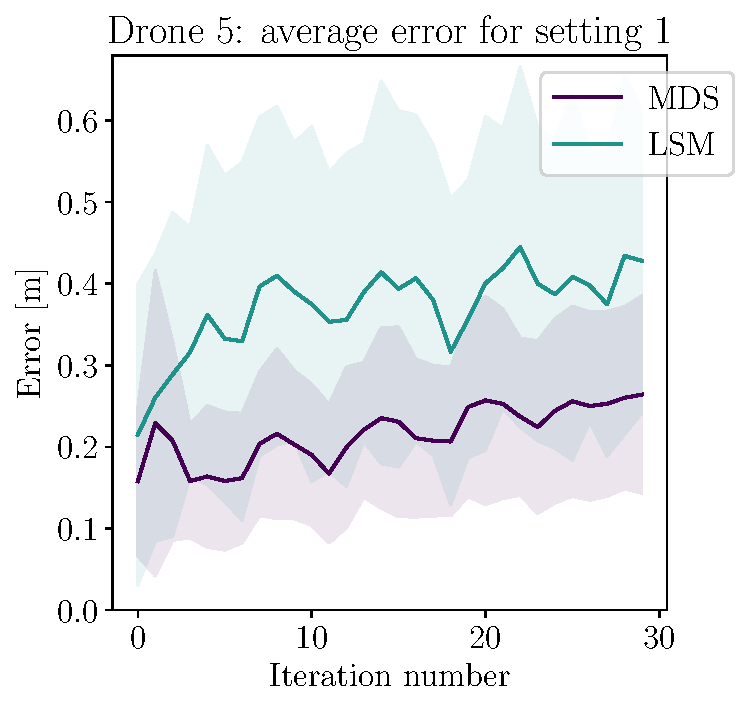
\includegraphics[width=\textwidth]{figures/drone5_setting1.pdf}
         \caption{Setting 1.}
         \label{fig:setting1_drone5}
     \end{subfigure}
     \hfill
     \begin{subfigure}[b]{0.28\textwidth}
         \centering
         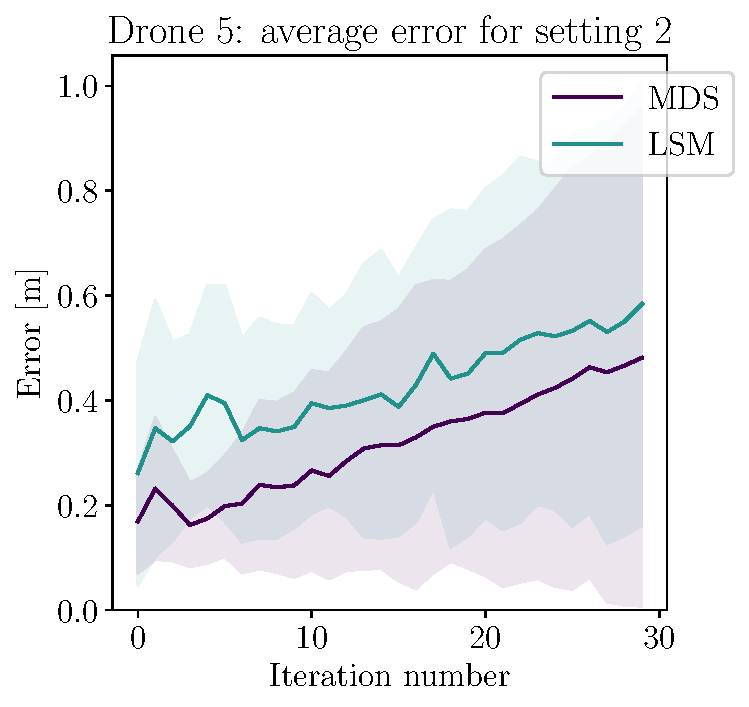
\includegraphics[width=\textwidth]{figures/drone5_setting2.pdf}
         \caption{Setting 2.}
         \label{fig:setting2_drone5}
     \end{subfigure}
     \hfill%
      \begin{subfigure}[b]{0.28\textwidth}
         \centering
         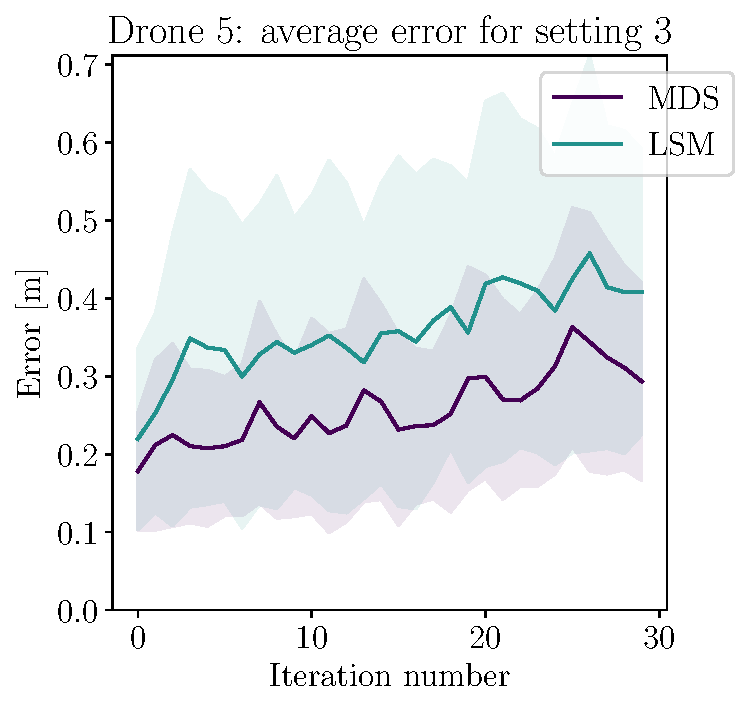
\includegraphics[width=\textwidth]{figures/drone5_setting3.pdf}
         \caption{Setting 3.}
         \label{fig:setting3_drone5}
     \end{subfigure}
     \hfill
     \begin{subfigure}[b]{0.28\textwidth}
         \centering
         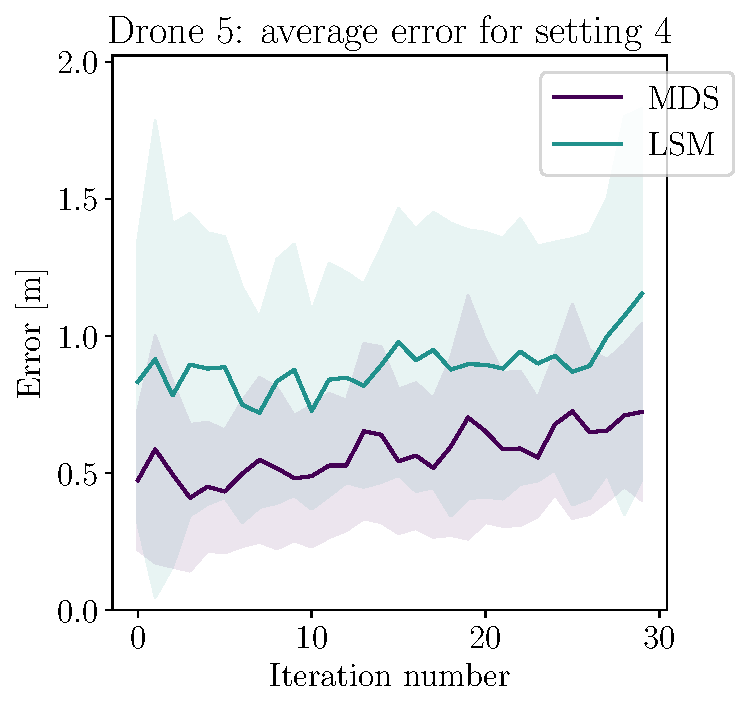
\includegraphics[width=\textwidth]{figures/drone5_setting4.pdf}
         \caption{Setting 4.}
         \label{fig:setting4_drone5}
     \end{subfigure}
     \hfill
     \begin{subfigure}[b]{0.28\textwidth}
         \centering
         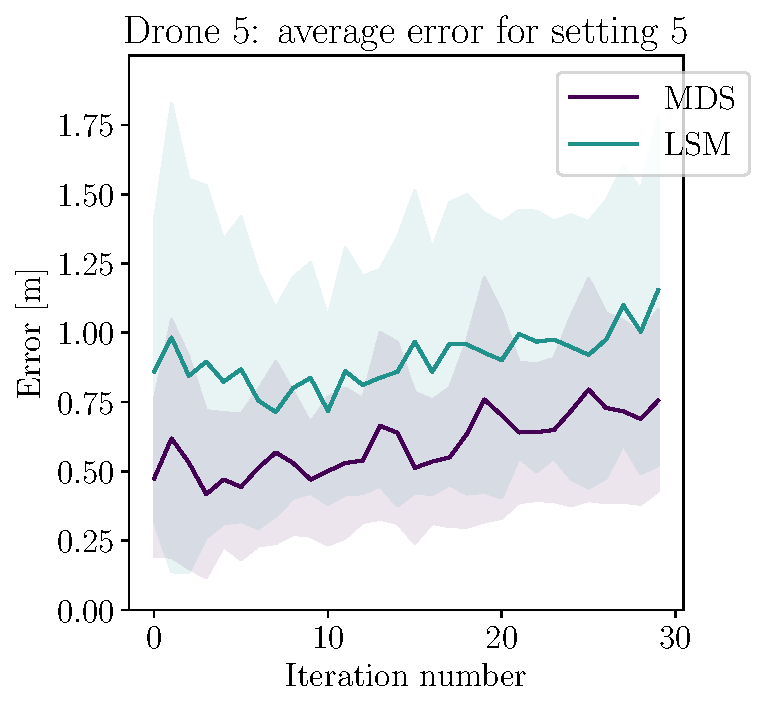
\includegraphics[width=\textwidth]{figures/drone5_setting5.pdf}
         \caption{Setting 5.}
         \label{fig:setting5_drone5}
     \end{subfigure}
     \hfill
     
     \caption[Drift]{
        \textbf{Drift.} 
        The five graphs illustrate the performances over time for the two considered algorithms. Specifically, the average estimation error and its trend for drone5 (chosen arbitrarily) is shown for the different tested settings. Independently, the average error always increases, highlighting the drift phenomenon. 
     }
     \label{fig:simulation_performances}
\end{figure*}

The comparison of different noises, based on the data collected, presents challenges due to varying attributes and quantity involved (e.g. distances, times, positions), but their effects are evident, especially for Setting 4 and Setting 5, observable respectively in Figure~\ref{fig:setting4_drone5} and Figure~\ref{fig:setting5_drone5}. \par

This outcome underlines the potential for enhancements in error mitigation strategies against noises and drifts, such as the introduction of global measurements or absolute re-calibration procedures, as elaborated in the last section. \par

% Finally, Figure~\ref{alg:MDS} offers a visual representation of this project's execution within the Gazebo environment. This portrayal highlights the project's competence in accurately estimating drone positions in real-time, particularly when operating within the Gazebo+Ardupilot framework. This environment closely mirrors real-world deployment conditions, further validating the potentiality of this work. \par

Table~\ref{tab:error_reduction} illustrates the great performances of MDS over trilateration. Indeed, the algorithm provided an error reduction between $24.4\%$ and $40.0\%$. A noticeable information is that an error reduction of about $33.7\%$ was achieved in Setting 5, namely the most noisy and complex scenario tested. This directly highlights the strong capabilities and reliability of MDS. \par           

However, few improvements could be introduced to obtain even higher results. First of all, different MDS versions could be integrated, to better overcome the different type of noise and reduce the computational times. Example of those are enhanced Multidimensional Scaling (eMDS) \cite{eMDS}, dynamic Multidimensional Scaling (dMDS) \cite{dMDS}, MDS-MAP or GM-MDS. \par

\begin{table}[!ht]
  \centering
    \begin{tabular}{l|c}
      \textbf{Configuration} & \textbf{Error reduction} \\\hline
      Setting1 & $40.0\%$ \\\hline
      Setting2 & $24.4\%$ \\\hline
      Setting3 & $26.5\%$ \\\hline
      Setting4 & $33.7\%$ \\\hline
      Setting5 & $33.7\%$ \\\hline
    \end{tabular}
    \caption[Average error reduction by relying on MDS algorithm]{
        \textbf{Average error reduction by relying on MDS algorithm}: in the table the reduction in the average error is shown, by relying on the MDS algorithm for drones coordinates estimation instead of standard trilateration algorithm.  
    }
    \label{tab:error_reduction}
\end{table}

Additionally, partially-connected swarms could be studied and implemented with the introduction of distributed MDS and distributed-weighted MDS (dwMDS), to better face the weakness or absence of intercommunication among the drones, due to the presence of obstacles. \par

Another interesting research is the integration of such simulation with Kalmann filters, to better estimate the position of drones via a measurement-update approach. In particular, the estimation of the covariance matrix associated to the location of each drone could be used to update more accurately the covariance in the filter, in order to take advantage of the best features of both the tools.